\chapter{Literature Review}
% \label{ch:relatedwork}
Over the past few years, Internet of Things or IoT, has had a significant impact in our lives.
It plays an important role whether it is a smartphone or a smarthome environment or just something 
as handy as a smartwatch. Different types of data is collected and exchanged among interconnected 
sensors/devices through modern communication network infrastructure connected by million of 
IoT nodes \cite{8123913,7598173,7879243,6774858,10.1145/2872332}. This direction of computing 
has already overtaken the traditional methods based on stationary computing \cite{8058399}. 
As a paradigm, IoT expresses that most physical devices, such as smart phones, smart watches and 
other embedded devices are interconnected with each other. These devices communicate with data 
centers and exchange information \textemdash all while adhering to their routine tasks \cite{7879243}. \\
Following various popular technologies these days, such as smart homes, smart grid and smart healthcare, 
IoT has become one of the essential components of people's home and workplace existence. It will 
continue to impact the daily life of people and its not just limited to technology. IoT has been reported 
to be one of the most important technologies that will impact US interests in 2025 \cite{7879243}. 
The number of interconnected physical devices has already transcended the human population for a couple 
years now. In 2012, there were 9 billion interconnected physical devices \cite{8058399}. This rapid increase 
in the number of mobile devices suggested that conventional centralized cloud computing would struggle 
to satisfy the Quality of Service (QoS) for many applications. However, with the introduction of 5G 
technology, edge computing becomes a viable and key solution to solve this issue \cite{7568592,7414384,6568922}. 
The edge computing platform allows edge nodes to respond to service demands which results in reduced 
bandwidth consumption and network latency. Figure \ref{fig:edgearch} shows a basic edge computing architecture. \\ 
\begin{figure}
    \begin{center}
        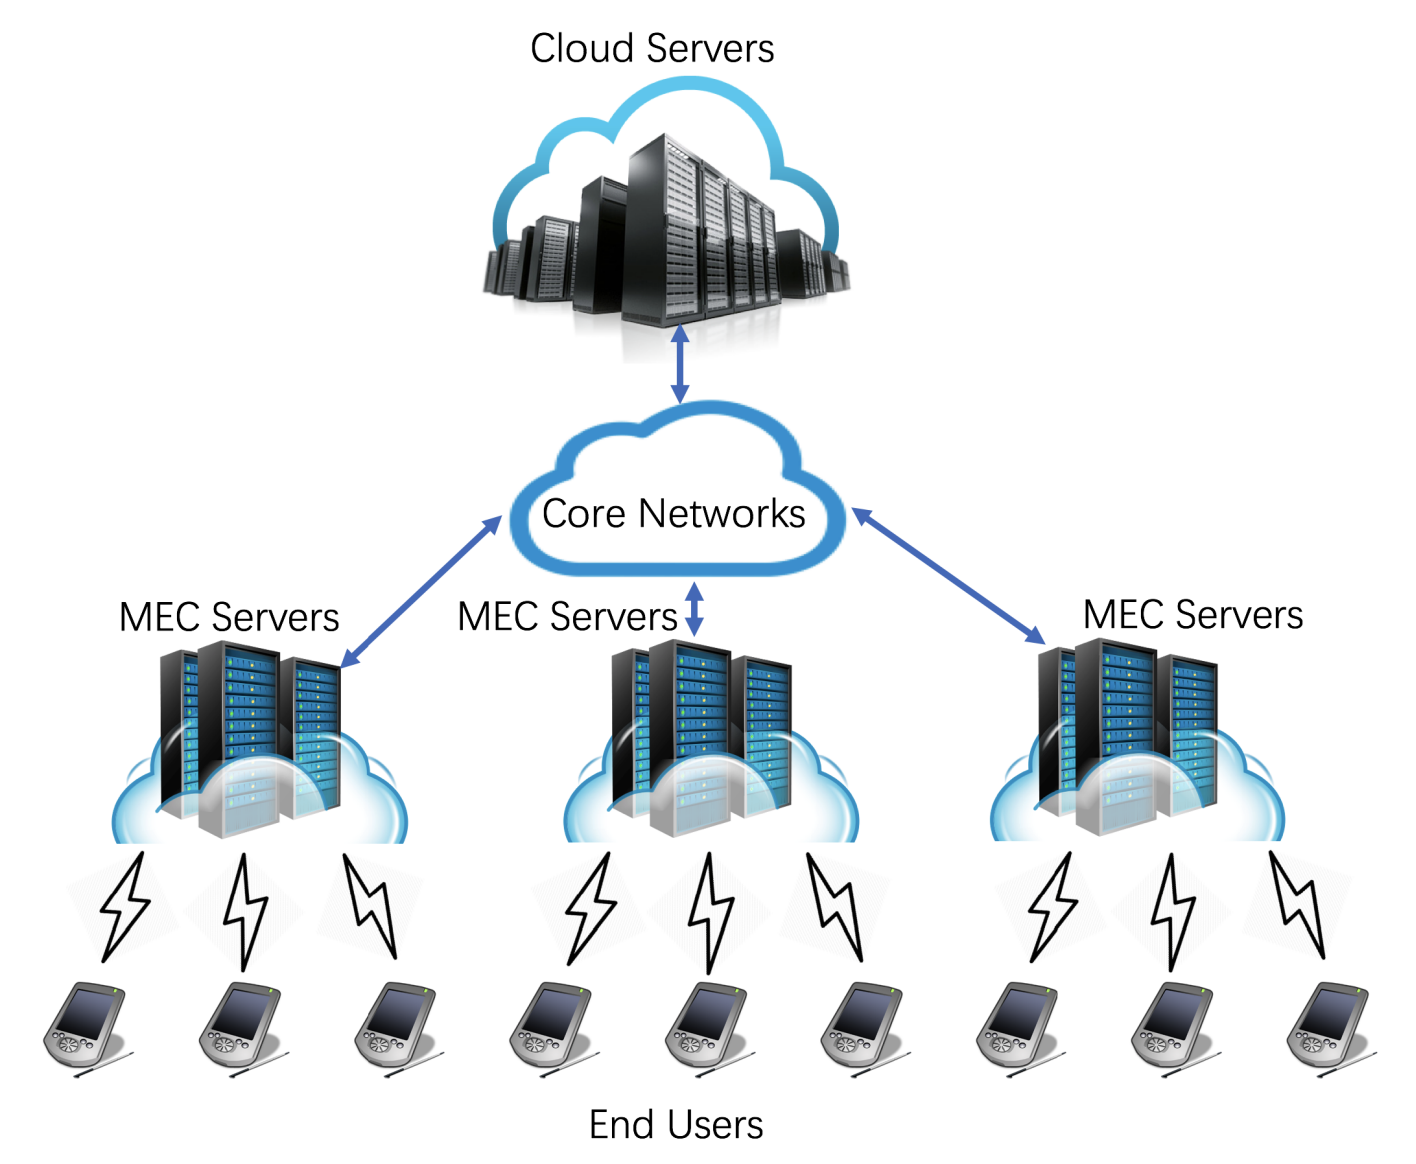
\includegraphics[scale=0.35]{Figs/edge_arch.png}    
    \end{center}
    \caption{The basic edge computing architecture}
    \label{fig:edgearch}
\end{figure}

Edge computing based IoT helps solve some critical issues and improves performance. Not to mention, IoT and 
edge computing share some characteristics which is further clarified by figure \ref{fig:edgeiot}. 
\begin{figure}
    \begin{center}
        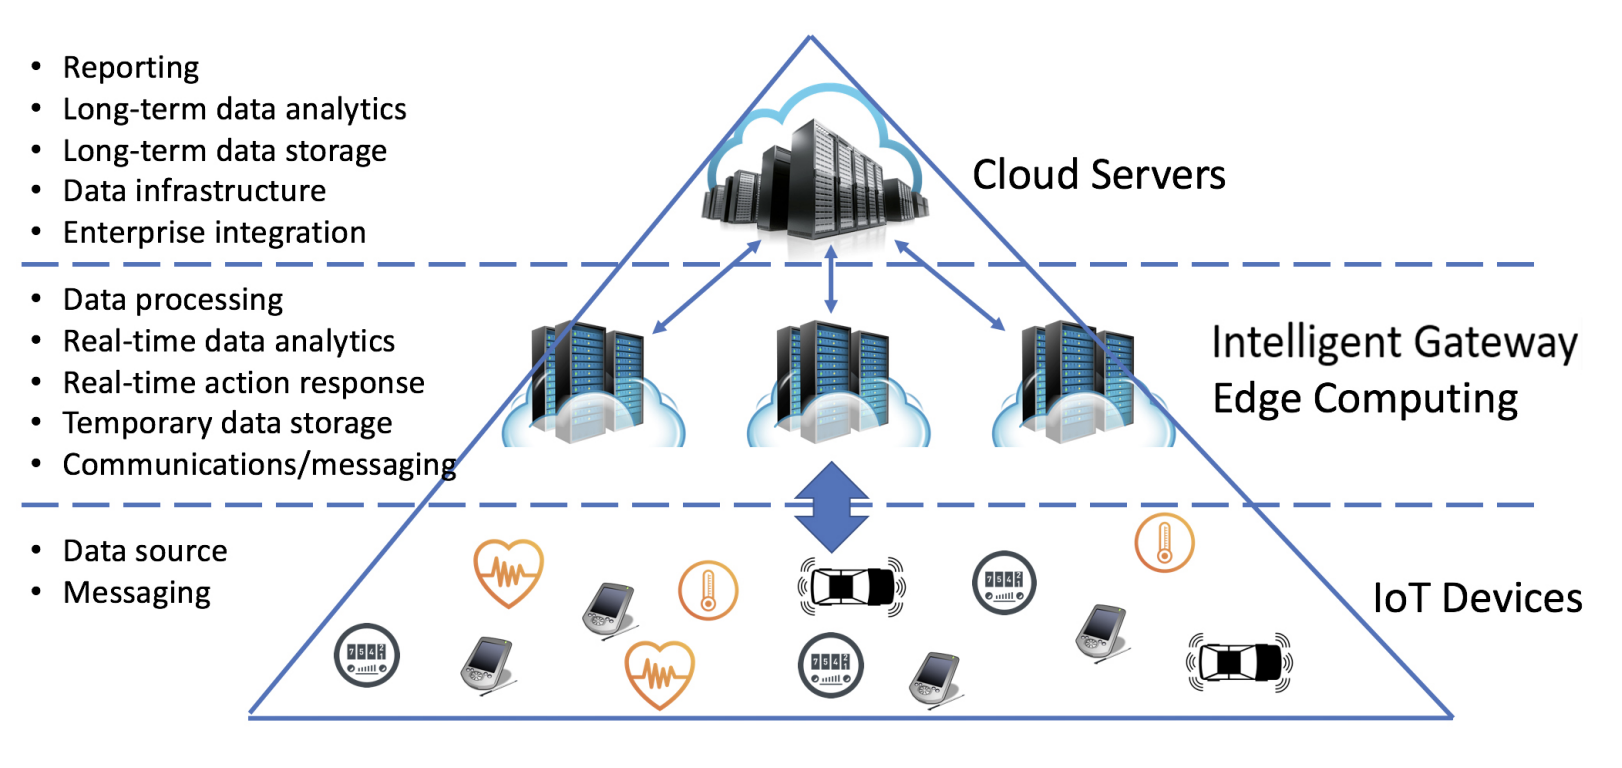
\includegraphics[scale=0.35]{Figs/edge_iot.png}    
    \end{center}
    \caption{Edge computing based IoT architecture}
    \label{fig:edgeiot}
\end{figure}

It further illustrates that IoT devices are end users for edge computing and IoT can benefit from both 
cloud and edge computing. The latter helps with faster response times and provides a tolerable computational 
capacity and storage space. Nowadays, the physical end user devices such as smart phones are considered 
edge devices. They may have an exclusively local component of an application but most generally, some sort of 
data is communicated with the cloud server, with or without the help of a gateway device. \\
One of the restricting factors among IoT edge devices is limited battery life (among limited storage and other things). 
Even though IoT and mobile devices are enabling  a connected future that promises huge amounts of time and money 
saved with better automation, control in industry and our everyday activities, as well as other benefits such as 
better health care via remote monitoring and efficient fuel usage in smart and increasingly autonomous vehicles \cite{9017997}, 
it is a matter of fact that amongst these are portable devices which require a battery to operate. Usually, these 
devices have small form factors which limits the size of battery that can be used in these devices. There haven't 
been dramatic improvements in terms of alternative, more reliable battery types which in turn limits the 
capabilities of components in such edge devices. Figure \ref{fig:energyphone} shows a breakdown of average energy usage across 
1520 users of Samsung Galaxy S3 and S4 mobile devices \cite{9017997}. In this experiment, users were divided into 
five groups based on their activity levels. It shows that each group of users has varying needs for which respective 
hardware component consumes more energy. In the recent years, there has been a strong motivation to minimize energy 
and power across all of these components so that mobile and IoT devices last longer on a single charge, and to also 
allow more sophisticated components such as CPU, GPUs and NPUs \cite{9017997}. \\

\begin{figure}
    \begin{center}
        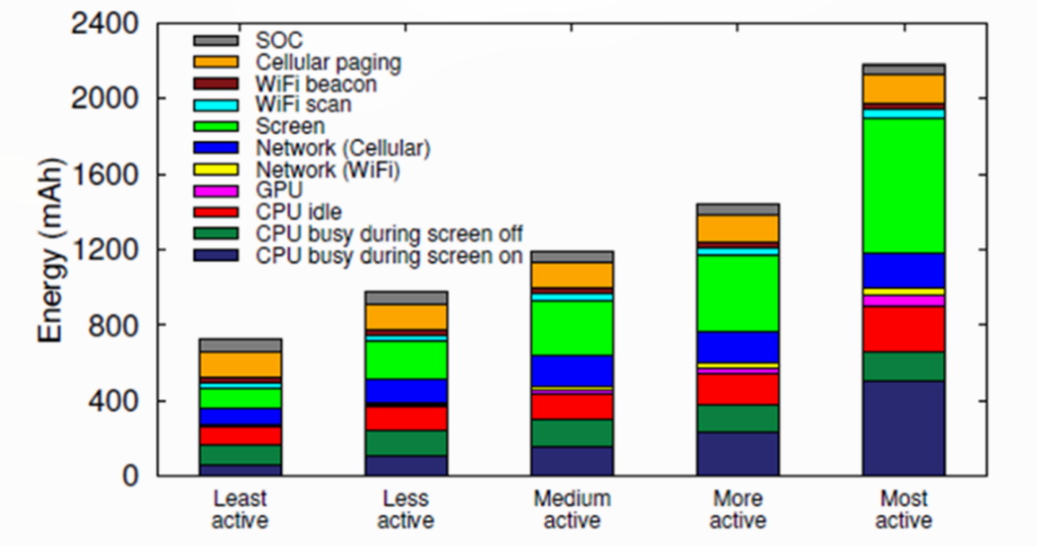
\includegraphics[scale=0.35]{Figs/energyphone.png}    
    \end{center}
    \caption{Average daily energy drain breakdown of 5 groups of 1520 apps \cite{9017997}}
    \label{fig:energyphone}
\end{figure}

This need of minimizing energy consumption of such devices had lead to a plethora of techniques being developed to 
reduce the overall energy consumption of edge devices. Researchers have used machine learning approaches to 
categorize applications during execution and choose a suitable pre-existing power plan \cite{power,7851469,4838819}. 
However, it was later realized that this does not capture dynamic workload variations \cite{5751506}. Later on, a new 
technique was proposed which involved phase level instrumentation to collect workload statistics at runtime. Essentially, 
the worload was divided into snippets and performance application programming interface calls were inserted between 
each snippet. The data collected from each snippet was then used to control the power states of processing elements \cite{dypo}. 
There are other ML based approaches as well where some are better than the other using Reinforcement Learning and 
Imitation Learning \cite{7092630,7163527,8449105,8607043,DBLP:journals/corr/abs-1011-0686,7934357,8770273}. Other than 
display optimations \cite{7544394,Dong2009PowersavingCT,187123}, wireless radio optimizations \cite{enloc,ener,min,delay,194920,180309} and 
main memory optimizations \cite{7266864}, there have also been software and user-centric optimizations. A variety of 
OS level energy management techniques have been  proposed in literature \cite{erdos,mob}. Runtime software profiling 
can identify the most power and energy hungry resournces that should be targetted by dynamic managament techniques. 
Powerscope \cite{powerscope} is one such example of a tool. It maps energy consumption of active applications to program 
structure. It further combines hardware instrumentation to measure current levels with kernel software support to 
perform statistical sampling of system activity. For mobile devices, the display is the main user interface. User 
satisfaction is directly impacted by brightness and content on the display. CAPED \cite{6972472} uses an online 
learning algorithm that dynamically controls the display brightness to meet individual user's preferences. Figure 
\ref{fig:onlinelearning} depicts how CAPED's online learning control works. \\

\begin{figure}
    \begin{center}
        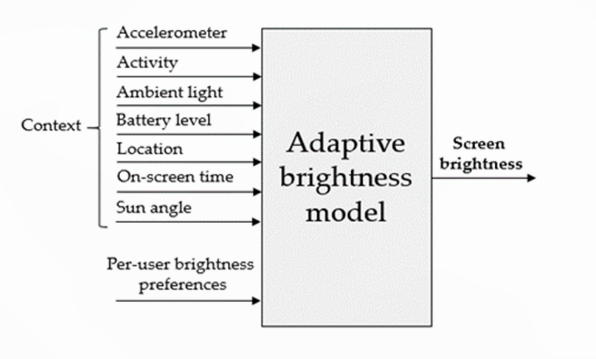
\includegraphics[scale=0.35]{Figs/online.png}    
    \end{center}
    \caption{Online learning control of display brightness \cite{6972472}}
    \label{fig:onlinelearning}
\end{figure}

Virtualization is commonly defined as the act of creating a virtual version of something, 
including but not limited to, hardware platforms, storage devices and network resources. It has many advantages 
including flexibility, capacity, processing power, growth in demand, and energy efficiency \cite{8360360}. A virtual 
machine instance represents an entire isolated environment. Multiple isolated environments can run and multiplex the 
resources of the same host. However, a new model has emerged which has been quite in demand for the past couple of years. 
\textit{Containers} \cite{turnbull_2014} allow multiple user-space instances and are generally lightweight. They have 
limited overhead compared to Virtual Machines (VMs) and unlike virtualization, paravirtualization or full virtualization, 
they do not require an emulation layer to run. Instead they use the host OS \cite{6903537}. One such notable example 
of a container framework is Docker \cite{turnbull_2014}. It unarguably started the container movement. Docker is open source 
system that provides an automated way to deplot applications inside containers \cite{8360360}. \\
Docker consists of multiple core components, described quite aptly by \cite{turnbull_2014}: 
\begin{itemize}
    \item \textbf{Docker client and daemon: }the client is basically a command-line binary which performs requests for the daemon. The daemon itself can either be run remotely or on the same host.
    \item \textbf{Docker images: }labelled as the \textquotedblleft source code \textquotedblright for the containers, images are the building blocks of Docker.
    \item \textbf{Registries: }used to store the images built. There are two types of registeries, public and private
    \item \textbf{Docker container: }applications and services are packaged inside containers. They are released from images and may contain one or more services.
\end{itemize}

Container performance is an important attribute to evaluate the quality of offered service. It represents 
system throughput, responsiveness, resource utilization, response time, latency, failure rate and fault 
tolerance \cite{perfcont}. With containers being very flexible and having the ability to fine tune specific metrics, 
the important question to ask is whether they can help preserve energy in certain scenarios. This will be further discussed 
in a later section. \\

Another technology that is quite interesting is edge based IoT middleware frameworks. One good example of is the 
Apache Cordova \cite{cordovahost}. A typical IoT middleware comprises of a three-layer architecture i.e. edge, gateway and cloud \cite{7582463}. 
A middleware is generally designed to be the intermediary between IoT devices and applications. The interaction is performed 
with the help of an \textit{accessor}. Accessors provide the abstraction for smart things across different hardware or 
software platforms to interact. They further allow for smarter interactions, sharing and portability. They are usually 
implemented in Javascript to keep it lightweight and ubiquitous, allowing things to communicate to share information 
in a message oriented fashion \cite{9446337}. An accessor has inputs, by which the swarmlet makes requests, and outputs, 
by which the service issues responses. The responses can be asynchronous and an accessor does not need to have an input; 
it can spontaneouly produce outputs \cite{7006378}. This is also depicted in Figure \ref{fig:accessor}. Accessor hosts function 
as a middleware service which is used to instantiate and execute accessors. They have their own specific set of actions 
that they can perform but the most common accessor hosts include Browser, Node and Cordova. The first supports 
executing accessors in a web browser whereas a Node host is just and Node.js engine with support for common host's 
capabilities \cite{9446337}. A Cordova host is an extension of the Apache Cordova's cross mobile program development 
platform. It is used for building application using basic web development elements such as HTML, CSS and JS, in a 
unified code base and targeted to multiple platforms like Android and IOS. Other than writing the plugin for the respective 
target device, no additional programming is required as its javascript interface interacts with native language APIs 
of physical or virtual IoT devices. 

\begin{figure}
    \begin{center}
        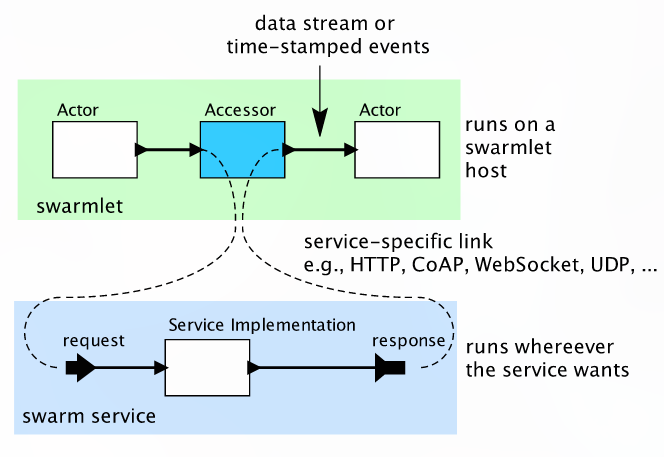
\includegraphics[scale=0.35]{Figs/accessor.png}    
    \end{center}
    \caption{Design pattern of accessors \cite{7006378}}
    \label{fig:accessor}
\end{figure}

The architecture of Cordova Accessor Host is given by Figure \ref{fig:cordova}. Briefly, it consists of a webview and 
a Cordova Plugin. Webview comprises of an implementation for the Common Host, an implementation for accessor host 
specific to Cordova and a bundle of all community developmed accessors that can be shared. This is what makes up the 
Cordova Accessor Host. The swarmlet.js component acts as an entry method, used to launch the accessor pipeline.

\begin{figure}
    \begin{center}
        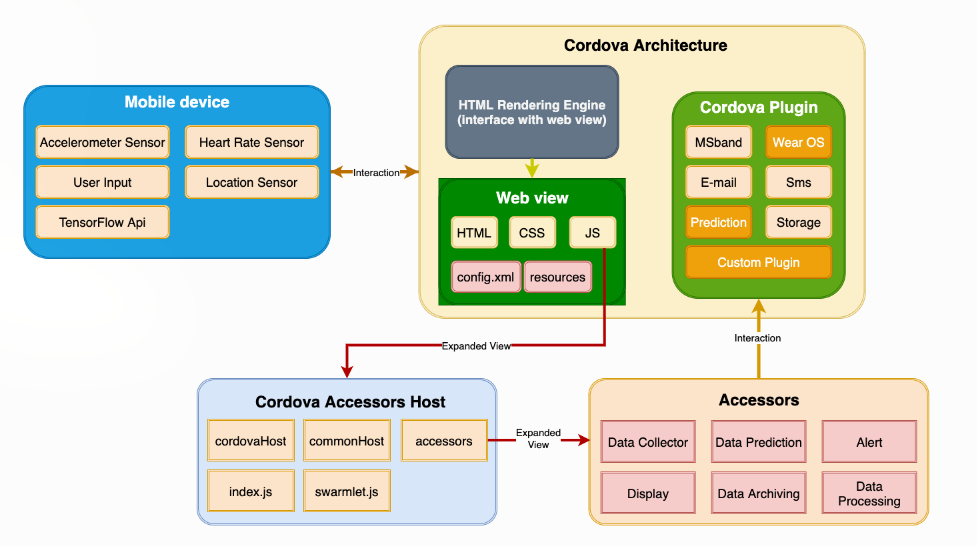
\includegraphics[scale=0.35]{Figs/cordova.png}    
    \end{center}
    \caption{Design pattern of accessors \cite{9446337}}
    \label{fig:cordova}
\end{figure}